
\subsection{Reynolds Transport Theorem}

Before stating and proving Reynolds Transport Theorem, we tackle the simpler
Leibniz integral rule. To gain some physical intuition on it, suppose we have a
very thin tube along the $x$--axis containing a fluid in motion. In this context
we may assume that the fluid only moves along the tube direction. Let $f =
f(x,t)$ be a magnitude of the fluid, for instance, the velocity $u$, the
temperature $T$ or the concentration of some chemical species $Y$. So as to
study how this magnitude variates on a portion of fluid, we consider a control
volume $U(t) = [a(t), b(t)]$ that depends upon time. This situation is picture
in figure \ref{fig:reynolds_transport_theorem_leibniz_rule}. The total ammount
of magnitude $f$ in the control volume at time $t$, which we will denote by
$\mathcal{F}(t)$, is given by
\begin{equation*}
	\mathcal{F}(t) = \int_{a(t)}^{b(t)} f(x,t) \dd{x}
\end{equation*}
and its rate of variation 
\begin{equation} \label{eq:reynolds_transport_theorem_motivation}
	\frac{\dd}{\dd{t}} \mathcal{F}(t) = 
	\frac{\dd}{\dd{t}} \int_{a(t)}^{b(t)} f(x,t) \dd{x}
\end{equation}

\begin{figure}[ht]
	\centering
	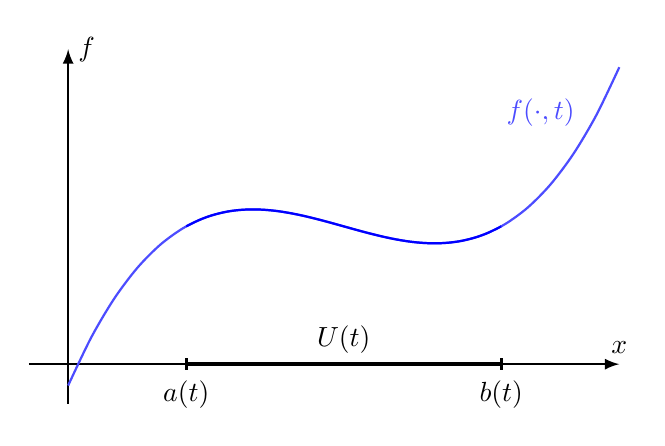
\begin{tikzpicture}
		\tikzset{
			brace/.style={
				decoration={brace, mirror},
				decorate
			}
		}
		% Axis
		\draw[-latex, thick] (-0.5,0) -- (7,0) node[above]{$x$};
		\draw[-latex, thick] (0,-0.5) -- (0,4) node[right]{$f$};
		% Control volume		
		\draw[very thick] (1.5,0.075) -- (1.5,-0.075) node[below]{$a(t)$};
		\draw[very thick] (5.5,0.075) -- (5.5,-0.075) node[below]{$b(t)$};
		\draw[very thick] (1.5,0) -- node[midway, above]{$U(t)$} (5.5,0);
		% Function f
		\draw[scale=1, domain=0:7, smooth, variable=\x, blue!70!white, thick]
		plot ({\x}, {0.07*(\x-1.5)*(\x-3.5)*(\x-5.5)+1.75});
		\draw[scale=1, domain=1.5:5.5, smooth, variable=\x, blue, thick]
		plot ({\x}, {0.07*(\x-1.5)*(\x-3.5)*(\x-5.5)+1.75});
		% Node
		\node[blue!70!white] at (6,3.2) {$f(\cdot,t)$};
	\end{tikzpicture}
	\caption{Control volume and magnitude $f$ at time $t$.}
	\label{fig:reynolds_transport_theorem_leibniz_rule}
\end{figure}

Computing the derivative in equation
\eqref{eq:reynolds_transport_theorem_motivation} can be difficult depending on
the case. Here is where Leibniz integral rule comes into play:

\begin{theorem}[Leibniz integral rule]
	Let $U \subset \real$ be a closed bounded interval and let $I = [t_1, t_2]$
	be the time interval. Let $a, b \colon I \rightarrow U$ be differentiable
	functions with continuous derivative. Let $f \colon U \times I \rightarrow
	\real$, $(x,t) \mapsto f(x,t)$ be a differentiable function such that
	$\pdv{f}{t}$ is also continuous. Then for all $t \in (t_1, t_2)$,
	\begin{equation*}
		\frac{\dd}{\dd{t}} \int_{a(t)}^{b(t)} f(x,t) \dd{x} = 
		\int_{a(t)}^{b(t)} \pdv{f}{t}(x,t) \dd{x} + f(b(t),t) b'(t) - f(a(t),t) a'(t)
	\end{equation*}
\end{theorem}
\begin{proof}
	See \cite{kaplan2002advanced}, Chap. 4, pg. 253--256.
\end{proof}

\noindent
Consider the more general case where we have a fluid in $n$--dimensional space
$\real^n$ and magnitude $f = f(x,t)$ defined on a control volume $\cvt \subset
\real^n$. The total ammount of $f$ on $\cv{}$ at time $t$ and its variation are given by similar formulas,
\begin{equation*}
	\mathcal{F}(t) = \int_\cvt f(x,t) \dd{x}, \quad
	\frac{\dd}{\dd{t}} \mathcal{F}(t) = \frac{\dd}{\dd{t}} \int_\cvt f(x,t) \dd{x}
\end{equation*}
however now computing the derivative might be impracticable. In this case we
have Reynolds Transport Theorem:

\begin{theorem}[Reynolds Transport Theorem \cite{kundu2008fluid}]
	Let $U \subset \real^n$ be a compact set (\ie $U$ is closed and bounded) and
	let $\cv{}(t)$ be a control volume depending on time such that $\cv{}
	\subset U$ for all $t \in I = [0, T]$ with $T > 0$. Let $\cs{}(t) = \partial
	\cv{}(t)$ be the boundary of $\cv{}(t)$ and let $F \in \mathcal{C}^1(U
	\times I, \real)$ be a scalar field. Then for all $t \in I$,
	\begin{equation*}
		\frac{\dd}{\dd{t}} \int_\cvt F(x, t) \dd{x} = 
		\int_\cvt \frac{\partial F}{\partial t} (x, t) \dd{x} + 
		\int_\cst F(x, t) \vb{b} \vdot \vb{n} \dd{S}
	\end{equation*}
	where $\vb{b} \colon \cs{}(t) \rightarrow \real^n$ is the local velocity of
	the control surface.
\end{theorem}
\begin{proof}
	The moving control volume $\cv{}(t)$ can be seen as the image of an initial
	region $\cv{}(0)$ by a family of $\mathcal{C}^1$ maps $\xi \colon U \times I
	\subset \real^n \times \real \rightarrow \real^n$, that is to say, $\cv{}(t)
	= \xi(\cv{}(0),t)$ for all $t \in I$. Furthermore, by fixing one time $t$,
	the mapping $\xi(\cdot, t) \colon \cv{}(0) \rightarrow \cv{}(t)$ can be
	assumed to be a diffeomorphism. Since $F$ is continuous, we can apply the
	Change of Variables Theorem taking $x = \xi(x_0,t)$,
	\begin{equation*}
		\int_\cvt F(x,t) \dd{x} = 
		\int_{\cv{}(0)} F(\xi(x_0,t), t) \abs{\det(\frac{\partial \xi}{\partial x_0} (x_0, t))} \dd{x_0}
	\end{equation*}
	where the determinant of the jacobian matrix $\det(\frac{\partial
	\xi}{\partial x_0} (x_0, t))$ can be assumed to be positive for
	small enough $T$, hence the absolute value is dropped. Applying
	differentiation under the integral sign (Theorem
	\ref{theo:differentiation_under_the_integral_sign}) with respect to $t$
	yields
	\begin{multline*}
		\frac{\dd}{\dd{t}} \int_\cvt F(x, t) \dd{x} = 
		\int_{\cv{}(0)} \pdv{t} 
		\left\{
		F(\xi(x_0,t), t) \ \det(\frac{\partial \xi}{\partial x_0} (x_0, t))
		\right\}
		\dd{x_0} 
		\\
		= 
		\int_{\cv{}(0)} 
		\pdv{t} \left\{ F(\xi(x_0,t), t) \right\} \det(\frac{\partial \xi}{\partial x_0} (x_0, t)) \dd{x_0} + 
		\int_{\cv{}(0)} F(\xi(x_0,t), t) \, \pdv{t} \left\{ \det(\frac{\partial \xi}{\partial x_0} (x_0, t)) \right\} \dd{x_0}
	\end{multline*}
	On the one hand,
	\begin{equation*}
		\pdv{t} \left\{ F(\xi(x_0,t), t) \right\} \det(\frac{\partial \xi}{\partial x_0} (x_0, t)) = 
		\left\{ 
		\frac{\partial F}{\partial t} (\xi(x_0, t), t) + 
		\grad{F(\xi(x_0, t), t)} \vdot \xi_t (x_0, t)
		\right\}
		\det(\frac{\partial \xi}{\partial x_0} (x_0, t))
	\end{equation*}
	where $\xi_t = \pdv{\xi}{t}$. On the other hand, using matrix calculus,
	\begin{equation*}
		F(\xi(x_0,t), t) \, \pdv{t} \left\{ \det(\frac{\partial \xi}{\partial x_0} (x_0, t)) \right\} = 
		F(\xi(x_0,t), t) \det(\frac{\partial \xi}{\partial x_0} (x_0, t)) \, \div{\xi_t(x_0,t)}
	\end{equation*}
	Thereby the integral is written as
	\begin{multline*}
		\frac{\dd}{\dd{t}} \int_\cvt F(x, t) \dd{x} = 
		\int_{\cv{}(0)} 
		\left\{
		\frac{\partial F}{\partial t} + \grad{F} \vdot \xi_t + F \div{\xi_t}
		\right\} \det(\frac{\partial \xi}{\partial x_0}) \dd{x_0} 
		\\ = 
		\int_{\cv{}(0)} 
		\left\{	\frac{\partial F}{\partial t} + \div(F \xi_t) \right\} \det(\frac{\partial \xi}{\partial x_0}) \dd{x_0}
	\end{multline*}
	So as to obtain an integral over $\cv{}(t)$, the previous change of
	variables is reverted, that is, $x_0 = \xi^{-1}(x, t)$. In order
	not to complicate notation, let $\vb{b}(x,t) =
	\xi_t(\xi^{-1}(x,t),t)$, then
	\begin{equation*}
		\frac{\dd}{\dd{t}} \int_\cvt F(x, t) \dd{x} = 
		\int_\cvt 
		\left\{ \frac{\partial F}{\partial t}  + \div(F \vb{b}) \right\} (x, t) \dd{x}
	\end{equation*}
	For a fixed $x_0 \in \cv{}(0)$, $\xi(x_0, \cdot)$ is a function of
	time giving how $x_0$ moves, hence $\xi_t(x_0, t)$ is the
	instantaneous velocity of $x_0$. To end, an application of divergence
	theorem yields the final formula:
	\begin{equation*}
		\frac{\dd}{\dd{t}} \int_\cvt F(x, t) \dd{x} = 
		\int_\cvt \frac{\partial F}{\partial t} (x, t) \dd{x} +
		\int_\cst F(x, t) \vb{b} \vdot \vb{n} \dd{S}
	\end{equation*}
\end{proof}







